\documentclass[fontsize=12pt]{scrartcl}
\usepackage[ngerman]{babel}
\usepackage[utf8]{inputenc}
%\usepackage[latin1]{inputenc}
\usepackage{amsmath}
\usepackage{amstext}
\usepackage{amssymb}
\usepackage{stmaryrd}
\usepackage{verbatim}
\usepackage{mathrsfs}
\usepackage{extarrows}
\usepackage[arrow, matrix, curve]{xy}
\usepackage[centering,includeheadfoot,margin=2cm]{geometry}
\usepackage{gensymb}
\usepackage{graphicx}
\usepackage{framed}
\usepackage{tabularx}
\usepackage{xcolor}
\usepackage{float}
\usepackage{graphicx} 
\usepackage{sidecap}
\usepackage{blindtext,wrapfig}
\usepackage{epstopdf}
\usepackage{import}
\usepackage{fancyhdr}
\usepackage{fancybox}
\usepackage{paralist}
\usepackage{graphicx}
\usepackage{caption}
\usepackage{subcaption}
\renewcommand{\l}{\left\vert}
\renewcommand{\r}{\right\vert}
\newcommand{\define}{\ensuremath{\mathrel{\mathop:}=}} % hübscheres :=, da = zentriert wird relativ zu :
\newcommand{\enifed}{\ensuremath{=\mathrel{\mathop:}}} % hübscheres =:, da = zentriert wird relativ zu :
\newcommand{\ddt}{\frac{\partial}{\partial t}}
\newcommand{\ddn}{\frac{\partial}{\partial N}}
\DeclareGraphicsRule{.tif}{png}{.png}{`convert #1 `basename #1 .tif`.png} 
\pagestyle{fancy}
\fancyhf{}
\fancyhead[R]{Physikalisches Praktikum 1}
\fancyfoot[R]{\thepage}
\fancyfoot[L]{\today}
\parindent 0pt
\parskip 12pt
\begin{document}

\begin{minipage}{0.9\textwidth}
\begin{center}\large
\title{ M42 Kreisel mit drei Achsen \\
		~\\
		~\\
		Assistent: Jonas Binz\\
		Datum Versuchsdurchführung: \\
		24.09.2015}

\author{bearbeitet von\\
		Gruppe: \\
		Gentian Rrafshi Matrnr. 2721617 \\
		Juliane Ratzsch Matrnr. 2967329}
\date{\today}

\maketitle

\end{center}
\end{minipage}

\newpage

\tableofcontents

\newpage
\noindent

\section{ Versuchsziel}

Ziel des Versuchs ist es das Trägheitsmoment eines Kreisels mit 3 Achsen und die Abhängigkeit der Nutationsfrequenz und Präzessionsfrequenz in Abhängigkeit zur Rotationsfrequenz zu bestimmen.

\section{ Grundlagen}

Grundlegend für den Versuch ist, dass eine Analogie zwischen Drehbewegung und Translation vorhanden ist. Diese sind:

\begin{figure}[H]
\centering
\begin{tabular}{|l l|l l|} \hline
 \multicolumn{2}{|c|}{Drehbewegung} &  \multicolumn{2}{c|}{Drehbewegung}\\ \hline
 Impuls &$ \vec{L} = J\cdot \vec{\omega}$ & Impuls & $\vec{p} = m \cdot \vec{v}$  \\
Drehmoment& $\vec{M}=\dot{\vec{L}}$ & Kraft & $\vec{F}=\dot{\vec{p}}$  \\
 Trägheitsmoment& $J = \int r^2$ d$m$& Masse & $m$  \\
 Strecke& $s$ & Winkel & $\varphi$  \\
 Winkelgeschwindigkeit& $\vec{\omega}$ & Geschwindigkeit & $\vec{v} $ \\ \hline
\end{tabular}
\end{figure} \par

Für einen Kreisel gilt, dass er ein starrer Körper ist. Desweiteren wird seine Drehbewegung genau dann symmetrisch genannt, wenn zwei Hauptträgheitsmomente identisch sind und wird kräftefrei genannt, wenn die äußeren Drehmomente sich aufheben. \par 

Ein senkrecht auf das Kreisel wirkende Drehmoment wird Präzession genannt, wenn das Drehmoment konstant bleibt. Bei nur  kurzer Einwirkung wird dies Nutation genannt. \par

Aus dem Drehmoment resultiert ein Drehimpuls. Dadurch, dass die Kraft nur senkrecht wirkt, ändert sich nur bei Präzession die Richtung, jedoch nicht der Betrag des Drehimpulses. Man erhält somit für den Kreisel eine Präzessionsfrequenz $\omega_\text{p}$ wie folgt:

\begin{align*}
\omega_{\text{p}} = \frac{M}{L} = \frac{\l \textbf{r} \times \textbf{F} \r}{J\omega}
\end{align*} \par 

Bei der Nutation entsteht eine Taumel- und Nickbewegung. Dies hat zur Folge, dass die Figurenachse und die Drehachse nicht mehr zusammenfallen, sonder um die Richtung des Drehimpulses rotieren.
\newpage

\section{Versuchsdurchführung}

\subsection{Versuchsbeschreibung}
\begin{figure}[H]
\centering
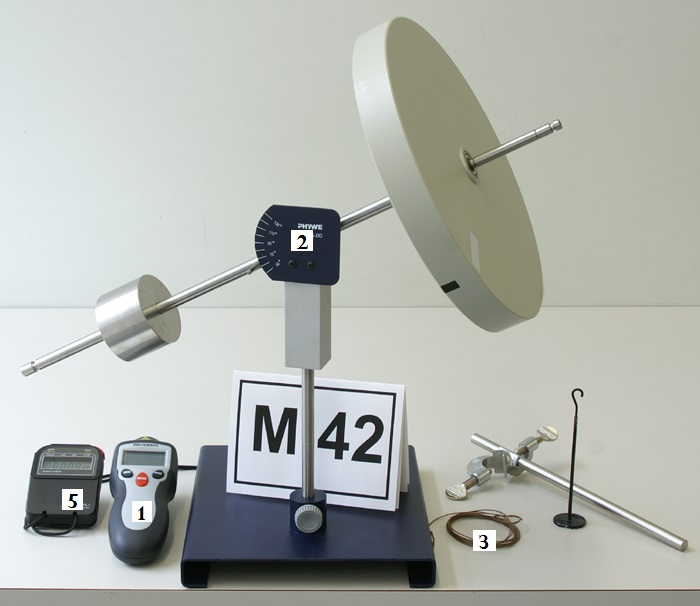
\includegraphics[width=0.5\textwidth]{Graphik/M42}
\caption{Versuchsskizze$^{\cite{A}}$}
\end{figure}

Für den Versuch werden folgende Gerätschaften benötigt:
\begin{itemize}
\item[1] Drehzahlmessgerät
\item[2] Kreisel mit 3 Achsen
\item[3] Faden
\item[4] Gewichte
\item[5] Stoppuhr
\end{itemize}

\newpage

\subsection{Versuchsablauf}

Im ersten Teil des Versuchs wird das Trägheitsmoment des Kreisels mit Hilfe der Winkelbeschleunigung bestimmt. Dazu wird die Kreiselachse horizontal ausgerichtet und eingespannt. An dem Faden wir ein Gewicht angehängt und an den Kreisel aufgespannt. Das Gewicht soll dann aus einer Höhe, welche die Unterkante des Tisches ist, losgelassen und die Fallzeit bis zum Boden wird gemessen, sowie die Drehzahl der Scheibe. Dieser Versuchsteil wird jeweils mit den Gewichten 160\,g und 110\,g 5 mal wiederholt. \par 

Im nächsten Teil des Versuchs soll das Kreisel auf etwa 400 bis 500 Umdrehungen pro Minute gebracht werde. Dann soll alle 5 Sekunden für 60 Sekunden die Drehzahl abgelesen werden.

Nun wird die Kreiselachse nicht mehr eingespannt, sondern mit Hilfe von Gegengewichten in horizontale Lage gebracht.  
Der freie Kreise wird nun aufgezogen und dem Gegengewicht ein weiteres Gewicht (10\,g und 60\,g) aufgehängt. Das Kreisel wird dann losgelassen und die Rotationsfrequenz jeweils am Anfang und am Ende der Drehung gemessen und über die Präzessionsdauer aufgetragen. Dies wird 10 mal ausgeführt, wobei die Rotationsfrequenz hier am Anfang zwischen 300 bis 800 Umdrehungen pro Minute liegen soll.

Zuletzt wird die Nutationsfrequenz ermittelt. Hierbei wird wieder der freie Kreisel aufgezogen und dem Kreisel wird mit ein seitlicher Schlag gegen die Kreiselachse eine Nutation gegeben. Nun wird die Zeit und die Rotationsfrequenz für 5 Nutationsumläufe am Anfang und Ende gemessen.  Diese Messung wird für 10 verschieden Rotationsfrequenzen im Bereich von 150 bis 500 Umdrehungen pro Minute durchgeführt.

\noindent
\newpage


\section{Formeln}

Für die Bestimmung des Trägheitsmomentes benötigen wir folgende Formel:

\begin{equation}
J = \frac{N}{\alpha} = \frac{\l r \times F \r}{\frac{\omega}{t}} = 	\frac{r \cdot m \cdot g \cdot t}{2 \cdot \pi \cdot n}
\label{j}
\end{equation}

Hierbei ist $J$ das Trägheitsmoment, $N$ Das Drehmoment, $\omega$ die Winkelgeschwindigkeit, $\alpha$ die Winkelbeschleunigung, $n$ die Drehzahl und $r$ der Radius der Kreisscheibe. \par

Eine weiter Formel ist die für die Präzessionsfrequenz:
\begin{equation}
\omega_{\text{p}} = \frac{N}{J\cdot \omega} = \frac{r \cdot m \cdot g}{J\cdot \omega}
\end{equation}
Woraus sich durch Umformen
\begin{equation}
\Rightarrow J = \frac{r \cdot m \cdot g}{\omega_{\text{p}}\cdot \omega}
\label{p}
\end{equation}
ergibt.\\
Die Variablenbezeichnungen sind identisch zu der von Formel (\ref{j}) mit $\omega_{\text{p}}$ als Präzessionsfrequenz.


\section{ Messwerte}
\begin{figure}[H]
\centering
\caption{Messwerte für direkte Messung des Trägheitsmoment}
\begin{tabular}{|c|c|c|} \hline
Gewicht [g] & Zeit [s] & Umdrehungen [$ \frac{1}{10\,\text{min}}$ ]  \\ \hline
160	&4,41	&1365  \\ \hline
160	&4,09	&1295 \\ \hline
160	&4,09	&1394 \\ \hline
160	&4,00	&1339 \\ \hline
160	&3,87	&1336 \\ \hline
110	&4,78	&1097 \\ \hline
110	&4,59	&1122 \\ \hline
110	&4,59	&1138 \\ \hline
110	&4,59	&1137 \\ \hline
110	&4,53	&1131 \\ \hline
\end{tabular}				 
\end{figure}
\begin{figure}[H]
\centering
\caption{Messwerte für die Abbremsung der Kreisscheibe}
\begin{tabular}{|c|c|c|c|} \hline
 Zeit [s] &  Umdrehungen [$ \frac{1}{10\,\text{min}}$ ] & Umdrehungen [$\frac{1}{10\,\text{min}}$ ]  & Umdrehungen [$\frac{1}{10\,\text{min}}$ ] \\ \hline
0		&4685	&4588	&4084 \\ \hline
5		&4500	&4367	&3888 \\ \hline
10	&4368	&4208	&3605 \\ \hline
15	&4151	&4088	&3549 \\ \hline
20	&3999	&3906	&3405 \\ \hline
25	&3888	&3765	&3282 \\ \hline
30	&3776	&3605	&3188 \\ \hline
35	&3365	&3477	&3031 \\ \hline
40	&3443	&3335	&2937 \\ \hline
45	&3214	&3214	&2813 \\ \hline
50	&3175	&3096	&2708 \\ \hline
55	&3062	&2949	&2606 \\ \hline
60	&2936	&2840	&2512 \\ \hline
\end{tabular}				 
\end{figure}
\begin{figure}[H]
\centering
\caption{Messwerte für die Präzessionsfrequenz der Kreisscheibe mit 10\,g Gegengewicht}
\begin{tabular}{|c|c|c|c|} \hline
Anfangsumdrehungen [$ \frac{1}{10\,\text{min}}$ ]  &  Endumdrehungen [$\frac{1}{10\,\text{min}}$ ]  &  Zeit [$s$] \\ \hline
4905	&3258	&42,00\\ \hline
3258	&2606	&27,00\\ \hline
2606	&2051	&21,28\\ \hline
2051	&1761	&18,22\\ \hline
5088	&3476	&44,57\\ \hline
3476	&2754	&33,78\\ \hline
2754	&2155	&23,00\\ \hline
2155	&1815	&18,72\\ \hline
6788	&4213	&56,74\\ \hline
4213	&3123	&33,35\\ \hline
3132	&2560	&28,53\\ \hline
2560	&2034	&20,50\\ \hline
7568	&4209	&57,00\\ \hline
\end{tabular}				 
\end{figure}
\begin{figure}[H]
\centering
\caption{Messwerte für die Präzessionsfrequenz der Kreisscheibe mit 60\,g Gegengewicht}
\begin{tabular}{|c|c|c|c|} \hline
Anfangsumdrehungen [$ \frac{1}{10\,\text{min}}$ ]  &  Endumdrehungen [$\frac{1}{10\,\text{min}}$ ]  &  Zeit [$s$] \\ \hline
6098	&5143	&10,70\\ \hline
9941	&8207	&14,41\\ \hline
8207	&7078	&13,87\\ \hline
7078	&6737	&12,16\\ \hline
6737	&6309	&9,81\\ \hline
6309	&5536	&8,13\\ \hline
5536	&5276	&8,35\\ \hline
4610	&4367	&7,77\\ \hline
4367	&4196	&7,00\\ \hline
7149	&6357	&12,22\\ \hline
\end{tabular}				 
\end{figure}
\begin{figure}[H]
\centering
\caption{Messwerte für die Nutationsfrequenz der Kreisscheibe}
\begin{tabular}{|c|c|c|c|} \hline
Anfangsumdrehungen [$ \frac{1}{10\,\text{min}}$ ]  &  Endumdrehungen [$\frac{1}{10\,\text{min}}$ ]  &  Zeit [$s$] \\ \hline
3573	&3281	&5,28\\ \hline
2784	&2602	&5,50\\ \hline
2876	&2494	&7,53\\ \hline
2420	&2227	&7,66\\ \hline
2784	&2602	&5,50\\ \hline
2128	&1952	&8,25\\ \hline
5610	&5115		&5,66\\ \hline
2134	&2003	&6,47\\ \hline
1651	&1402	&10,68\\ \hline
\end{tabular}				 
\end{figure}

\newpage

\section{ Auswertung}

\subsection{Auswertung Trägheitsmoment}
Im ersten Teil soll das Trägheitsmoment der Kreisscheibe berechnet werden. Dafür wird für die beiden Gewichte (160\,g und 110\,g) der Mittelwert der Umdrehungen gebildet, was wie folgt aussieht:
\begin{align*}
\bar{N}_{160} = \sum_{j=1}^{5} \frac{N_j}{5} = 2 \pi \cdot \frac{1365+1295+1394+1339+1336}{5\cdot 10 \cdot 60 }{\frac{1}{\text{s}}} = 14,09\,{\frac{1}{\text{s}}}
\end{align*}

und der Mittelwert der Zeit ist daher:
\begin{align*}
\bar{t}_{160} = \sum_{j=1}^{5} \frac{t_j}{5} =  \frac{(4,41+4,09+4,09+4,00+3,87)\,{\text{s}}}{5} = 4,09\,{\text{s}}
\end{align*}

Für 100\,g ergibt sich $\bar{N}_{110} = 11,78\,{\text{kg}\cdot{\text{m}^2}}$ und $\bar{t}_{110}=4,62$\,s.

Damit ergibt sich dann mit Hilfe von Formel (\ref{j}) folgendes:
\begin{align*}
J_{160} &=\frac{r \cdot m \cdot g \cdot \bar{t}_{160}}{\bar{N}_{160}} =	\frac{0,0225\,{\text{m}} \cdot 0,11\,{\text{kg}} \cdot 9,81\,\frac{ {\text{m}}}{{\text{s}^2}} \cdot 4,09\,{\text{s}}}{14,09\,{\frac{1}{\text{s}}}} \\&= 0,001025\,{{\text{kg} \cdot {\text{m}^2}}} = 10,25 \cdot 10^{-3}\,{{\text{kg} \cdot {\text{m}^2}}}
\end{align*}

und analog dazu folgt $J_{110} = 9,51\cdot 10^{-3}\,{{\text{kg} \cdot {\text{m}^2}}}$. 

Wir erhalten also folgende Werte: 
\begin{figure}[H]
\centering
\caption{Messwerte für direkte Messung des Trägheitsmoment}
\begin{tabular}{|c|c|c|} \hline
Gewicht [g] & Trägheitsmoment $J$ [$10^{-3}\cdot {{\text{kg} \cdot {\text{m}^2}}}$]  \\ \hline
160 & 10,25 \\ \hline
110 & 9,51\\ \hline
\end{tabular}				 
\end{figure}

\newpage

\subsection{Auswertung Dämpfungskonstante}

Hierbei muss erstmal unsere Umdrehung von $\frac{10}{\text{min}}$ auf $\frac{1}{\text{s}}$ gebracht werden. Dies wird anhand eines Beispiels vorgerechnet:
\begin{align*}
4685\,\frac{1}{10 \text{min}} = 468,5\,\frac{1}{ \text{min}} = 7,81\,\frac{1}{ \text{s}}
\end{align*}
Die nachfolgende Tabelle enthält nun alle anderen ausgerechnete Werte:
\begin{figure}[H]
\centering
\caption{Auswertung für die Abbremsung der Kreisscheibe}
\begin{tabular}{|c|c|c|c|} \hline
 Zeit [s] &  Umdrehungen [$ \frac{1}{ \text{s}}$] & Umdrehungen [$ \frac{1}{ \text{s}}$]  & Umdrehungen [$ \frac{1}{ \text{s}}$] \\ \hline
0		&7,81	&7,65	&6,81 \\ \hline
5		&7,50	&7,28	&6,48 \\ \hline
10	&7,28	&7,01	&6,01 \\ \hline
15	&6,92	&6,81	&5,92 \\ \hline
20	&6,67	&6,51	&5,68 \\ \hline
25	&6,48	&6,28	&5,47 \\ \hline
30	&6,29	&6,01	&5,31 \\ \hline
35	&5,61	&5,80	&5,05 \\ \hline
40	&5,74	&5,56	&4,90 \\ \hline
45	&5,36	&5,36	&4,69 \\ \hline
50	&5,29	&5,16	&4,51 \\ \hline
55	&5,10	&4,92	&4,34 \\ \hline
60	&4,89	&4,73	&4,19 \\ \hline
\end{tabular}				 
\end{figure}
\newpage
Diese Werte werden nun geplottet. Es ergibt sich folgendes Diagramm:
\begin{figure}[H]
\centering
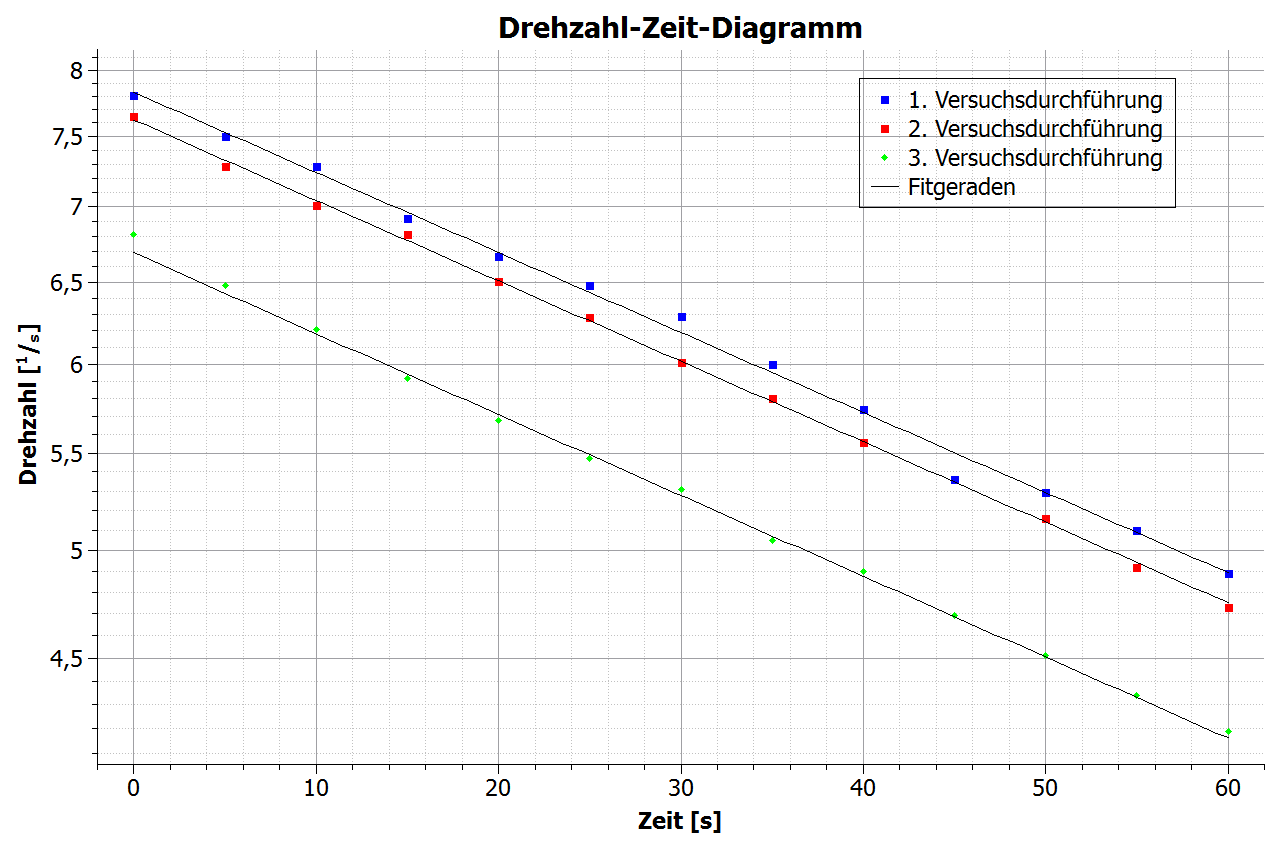
\includegraphics[width=0.95\textwidth]{Graphik/Drehzahlzeit}
\caption{Drehzahl-Zeit-Diagramm}
\end{figure}

Dadurch erhält man durch den Fitansatz $f(x)=A\cdot\exp(-kx)$ folgende Dämpfungen:
\begin{figure}[H]
\centering
\caption{Auswertung für die Abbremsung der Kreisscheibe}
\begin{tabular}{|c|c|c|c|} \hline
Versuchsreihe & Dämpfungskonstante [$10^{-3}$/s] \\ \hline
1 & 7,83 \\ \hline
2&  7,88 \\ \hline
3& 7,91 \\ \hline
\end{tabular}				 
\end{figure}
\newpage

\subsection{Trägheitsmoment bei Präzession}

Wenn wir in Formel (\ref{p})  $\omega_{\text{p}}=\frac{2\pi}{T}$  einsetzen, erhalten wir:
\begin{align*}
\omega_{\text{p}}&=\frac{2\pi}{T}=\frac{r \cdot m \cdot g}{J\cdot \omega} =\frac{r \cdot m \cdot g}{J\cdot \omega} \\
&\Rightarrow T= \frac{2\pi\cdot J\cdot\omega}{r\cdot m\cdot g} \\
&\Rightarrow \omega= \frac{r\cdot m\cdot g\cdot T}{2\pi\cdot J}
\end{align*}
Beim Auftragen ergeben sich folgende Diagramme für uns:
\begin{figure}[H]
\centering
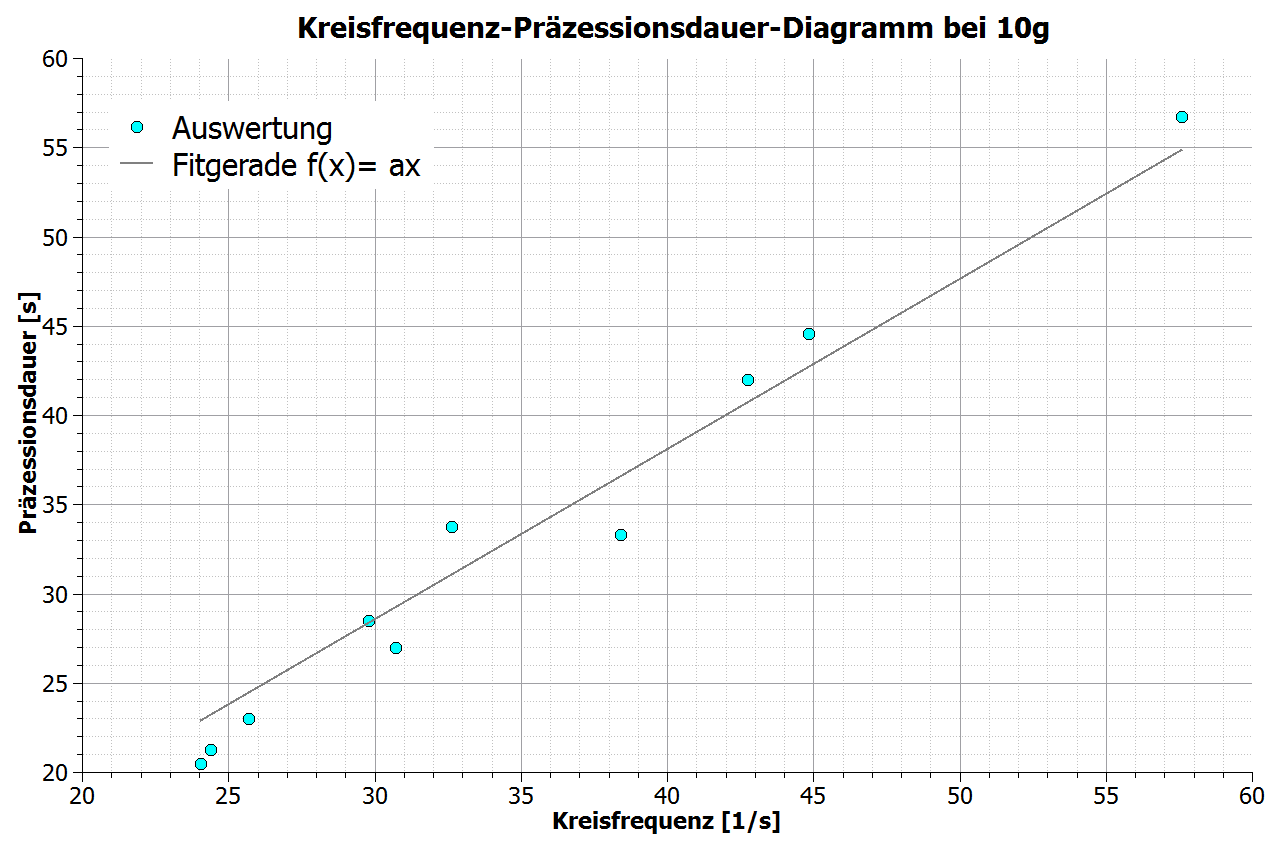
\includegraphics[width=0.65\textwidth]{Graphik/10g}
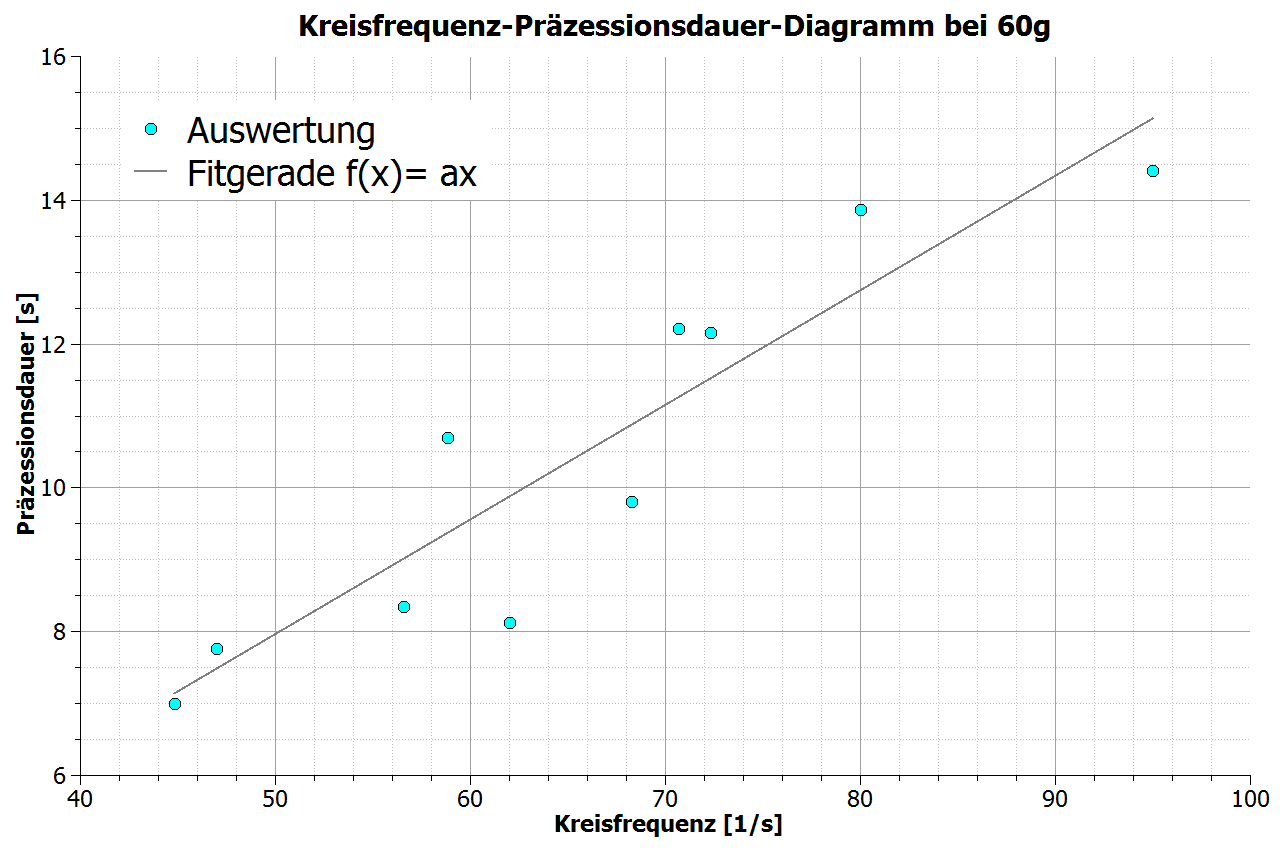
\includegraphics[width=0.65\textwidth]{Graphik/60g}
\caption{Rotationsfrequenz-Zeit-Diagramm}
\end{figure}
Tragen wir die Rotationsfrequenz gegen die Präzessionsdauer auf, so erhalten wir als Steigung 
\begin{figure}[H]
\centering
\caption{Auswertung Steigung für Trägheitsmoment bei Präzession}
\begin{tabular}{|c|c|c|c|} \hline
Gewicht & Steigung [s$^{-2}$] \\ \hline
10 & 0,95 \\ \hline
60 & 0,16  \\ \hline
\end{tabular}				 
\end{figure}
Woraus sich folgendes ergibt:
\begin{align*}
A_{10\,\text{g}}&= \frac{r\cdot m\cdot g}{2\pi\cdot J}\\
~\\
 \Rightarrow J&= \frac{r\cdot m\cdot g}{2\pi\cdot A_{10\,\text{g}}}\\
~\\
 J&=  \frac{0,27\,{\text{m}} \cdot 0,01\,{\text{kg}} \cdot 9,81\,\frac{{\text{m}}}{{\text{s}^2}}}{2\pi\cdot A_{10\,\text{g}}} =  \frac{4,22\,\frac{10^{-3}\,\text{kg}{\text{m}^2}}{{\text{s}^2}} }{0,95\,\text{s}^{-2}}= 4,43\cdot 10^{-3}  \text{kg}{\text{m}^2}
\end{align*}
bzw.
\begin{align*}
A_{60\,\text{g}}&= \frac{r\cdot m\cdot g}{2\pi\cdot J}\\
~\\
 \Rightarrow J&= \frac{r\cdot m\cdot g}{2\pi\cdot A_{60\,\text{g}}}\\
~\\
 J&=  \frac{0,27\,{\text{m}} \cdot 0,06\,{\text{kg}} \cdot 9,81\,\frac{{\text{m}}}{{\text{s}^2}}}{2\pi\cdot A_{60\,\text{g}}} =  \frac{25,29\,\frac{10^{-3}\,\text{kg}{\text{m}^2}}{{\text{s}^2}} }{0,16\,\text{s}^{-2}}=158,06\cdot 10^{-3}\,\text{kg}{\text{m}^2}
\end{align*}

In der nachfolgenden Tabelle werden dann zur dem Gewicht die entsprechende Steigung und das entsprechende Trägheitsmoment angegeben:
\begin{figure}[H]
\centering
\caption{Auswertung für Trägheitsmoment bei Präzession}
\begin{tabular}{|c|c|c|c|} \hline
Gewicht & Steigung [s$^{-2}$]& Trägheitsmoment $J$ [$10^{-3}$\,kg $\cdot$ m$^2$] \\ \hline
10 & 0,95 & 4,43  \\ \hline
60 & 0,16 & 158,06 \\ \hline
\end{tabular}				 
\end{figure}

\newpage

\subsection{Auswertung bei Nutation}

Im letzten Teil des Versuchs soll lediglich die Nutationsfrequenz über die Rotationsfrequenz aufgetragen werden. Beispielhaft wird hier die Nutationsfrequenz einmal für $T=5,5$\,s ausgerechnet. Die restlichen Werte werden dann in der danach folgenden Tabelle dargestellt und dann wird das Diagramm gezeigt.
\begin{align*}
\omega_{\text{Nut}} = \frac{2\pi \cdot 5}{T} =  \frac{10\pi }{5,5\,\text{s}} = 5,95\,\frac{1}{\text{s}}
\end{align*}
Damit ergibt sich:
\begin{figure}[H]
\vspace{-24pt}
\centering
\caption{Nutation}
\begin{tabular}{|c|c|c|c|} \hline
Zeit [s]& Nutationsfrequenz  [s$^{-1}$] & Rotationsfrequenz  [s$^{-1}$] \\ \hline
5,28	&5,95	&35,87\\ \hline
5,50	&5,71	&28,19\\ \hline
7,53	&4,17	&28,10\\ \hline
7,66	&4,10	&24,32\\ \hline
5,50	&5,71	&28,19\\ \hline
8,25	&3,81	&21,35\\ \hline
5,66	&8,55	&56,13\\ \hline
6,47	&4,85	&21,65\\ \hline
10,68 &2,94	&15,98\\ \hline
\end{tabular}				 
\end{figure}

und somit erhält man folgenden Plot:
\begin{figure}[H]
\centering
\includegraphics[width=0.75\textwidth]{Graphik/Nut}
\caption{Rotationsfrequenz-Zeit-Diagramm}
\end{figure}

\section{Fehlerrechnung}

\subsection{Fehlerquellen}

Es gibt hier wenige Fehlerquellen. Die ein Fehlerquelle ist das Drehzahlmessgerät, welches manchmal einfach nichts so wollte. Eine weitere Fehlerquelle ist dann noch die Zeitmessung, welche nun mal der menschlichen Reaktionszeit ausgesetzt ist. 

\subsection{Fehler Trägheitsmoment}

Aus Formel (\ref{j}) können wir eine Fehlerabschätzung machen, in der wir für $\Delta T= 1$\,s annehmen und für die Umdrehung $\Delta n = 60\,\frac{1}{10\,\text{min}}$ annehmen. Für $\Delta n$ ergibt sich dann, dass $\Delta n = 0,1\,\frac{1}{\text{s}}$ ist.

Damit ergibt sich bei uns:
\begin{align*}
\Delta J_{160} &=\l \ddt \frac{r \cdot m \cdot g \cdot \bar{t}_{160}}{\bar{N}_{160}}  \r  \cdot  \Delta T +\l \ddn \frac{r \cdot m \cdot g \cdot \bar{t}_{160}}{\bar{N}_{160}}  \r \cdot \Delta n \\
&= \l \frac{r \cdot m \cdot g}{\bar{N}_{160}} \r  \cdot  \Delta T +\l- \frac{r \cdot m \cdot g \cdot \bar{t}_{160}}{\bar{N}_{160}^2} \r \cdot \Delta n \\
&= \l \frac{0,0225\,{\text{m}} \cdot 0,16\,{\text{kg}} \cdot 9,81\,\frac{ {\text{m}}}{{\text{s}^2}}}{14,09\,{\frac{1}{\text{s}^2}}} \r  \cdot 1\,\text{s} +\l- \frac{0,0225\,{\text{m}} \cdot 0,16\,{\text{kg}} \cdot 9,81\,\frac{ {\text{m}}}{{\text{s}^2}} \cdot 4,09\,{\text{s}}}{(14,09\,{\frac{1}{\text{s}^2}})^2} \r \cdot 0,1\,\frac{1}{\text{s}} \\
&=2,58 \cdot 10^{-3}\,\text{kg m$^2$}
\end{align*}
und 
\begin{align*}
\Delta J_{110} &=\l \ddt \frac{r \cdot m \cdot g \cdot \bar{t}_{110}}{\bar{N}_{110}}  \r  \cdot  \Delta T +\l \ddn \frac{r \cdot m \cdot g \cdot \bar{t}_{110}}{\bar{N}_{110}}  \r \cdot \Delta n \\
&= \l \frac{r \cdot m \cdot g}{\bar{N}_{110}} \r  \cdot  \Delta T +\l- \frac{r \cdot m \cdot g \cdot \bar{t}_{110}}{\bar{N}_{110}^2} \r \cdot \Delta n \\
&= \l \frac{0,0225\,{\text{m}} \cdot 0,11\,{\text{kg}} \cdot 9,81\,\frac{ {\text{m}}}{{\text{s}^2}}}{11,78\,{\frac{1}{\text{s}^2}}} \r  \cdot 1\,\text{s} +\l- \frac{0,0225\,{\text{m}} \cdot 0,11\,{\text{kg}} \cdot 9,81\,\frac{ {\text{m}}}{{\text{s}^2}} \cdot 4,62\,{\text{s}}}{(11,78\,{\frac{1}{\text{s}^2}})^2} \r \cdot 0,1\,\frac{1}{\text{s}} \\
&=2,14 \cdot 10^{-3}\,\text{kg m$^2$}
\end{align*}

\newpage

\subsection{Fehler Dämpfungskonstante}

Bei dem Fit mit der Funktion $f(x) = A \cdot \exp (-kx)$ gibt uns Qti-Plot folgenden Fehler aus:

\begin{figure}[H]
\centering
\caption{Fehler Dämpfungskonstante}
\begin{tabular}{|c|c|c|c|c|} \hline
& Konstante $A$ [1/s] & Fehler  $\Delta A$ [$10^{-3}$/s]  & Konstante $k$ [$10^{-3}$/s] & Fehler  $\Delta k$ [$10^{-5}$/s] \\ \hline
 1 &  7,83 & 34,95& 7,83 & 14,85\\ \hline
 2 & 7,62 & 15,40 & 7,88 & 6,66\\ \hline
 3 &   6,69 & 39,35 & 7,91 & 18,77\\ \hline
\end{tabular}				 
\end{figure}
Wobei hier dann $k$ unsere Dämpfungskonstante ist.

\subsection{Fehler bei der Präzession}

Aus Qti-Plot erhalten wir die Fehler von $A_{\text{60g}}$ und $A_{\text{10g}}$. Die sind:
\begin{align*}
\Delta A_{\text{10g}} = 0,02\,\text{s}^{-2} \\
\Delta A_{\text{60g}} =0,02\,\text{s}^{-2}
\end{align*} 

Einsetzen ergibt dann:
\begin{align*}
\Delta J_{10\,\text{g}}&= \l \frac{\partial}{\partial A}  \frac{4,22\,\frac{10^{-3}\,\text{kg}{\text{m}^2}}{{\text{s}^2}} }{A_{10\,\text{g}}} \r \cdot \Delta
A_{10\,\text{g}} =  \frac{4,22\,\frac{10^{-3}\,\text{kg}{\text{m}^2}}{{\text{s}^2}} }{(0,95\,\text{s}^{-2})^2} \cdot  0,02\,\text{s}^{-2} = 0,10\cdot 10^{-3}  \text{kg}{\text{m}^2} \\
~\\
\Delta J_{60\,\text{g}}&= \l \frac{\partial}{\partial A}  \frac{25,29\,\frac{10^{-3}\,\text{kg}{\text{m}^2}}{{\text{s}^2}} }{A_{60\,\text{g}}} \r \cdot \Delta
A_{60\,\text{g}} =  \frac{25,29\,\frac{10^{-3}\,\text{kg}{\text{m}^2}}{{\text{s}^2}} }{(0,16\,\text{s}^{-2})^2} \cdot  0,02\,\text{s}^{-2} = 19,73\cdot 10^{-3}  \text{kg}{\text{m}^2}
\end{align*}


\newpage
\section{Zusammenfassung}

Im ersten Teil des Versuchs sollten wir direkt das Trägheitmoment der Kreisscheibe ausfindig machen.  Für uns ergaben sich folgende Werte mit folgenden Fehlern: 
\begin{figure}[H]
\centering
\caption{Zusammenfassung für direkte Messung des Trägheitsmoment}
\begin{tabular}{|c|c|c|} \hline
Gewicht [g] & Trägheitsmoment $J$ [$10^{-3}\cdot {{\text{kg} \cdot {\text{m}^2}}}$]  & Fehler $\Delta J$ $[10^{-3}\,\text{kg m$^2$}$]\\ \hline
160 & 10,25 & $\pm$ 2,58   \\ \hline
110 & 9,51 &  $\pm$ 2,14  \\ \hline
\end{tabular}				 
\end{figure}

Danach sollten wir die Dämpfungskonstante bestimmen. Auch hier werden die Werte nochmal zusammengefasst dargestellt:

\begin{figure}[H]
\centering
\caption{Zusammenfassung für die Abbremsung der Kreisscheibe}
\begin{tabular}{|c|c|c|c|} \hline
Versuchsreihe & Dämpfungskonstante $k$ [$10^{-3}$/s]  & Fehler $\Delta k$ [$10^{-5}$/s]\\ \hline
1 & 7,83 & $\pm$ 14,85 \\ \hline
2&  7,88 & $\pm$ 6,66\\ \hline
3& 7,91 & $\pm$	 18,77 \\ \hline
\end{tabular}				 
\end{figure}

Im dritten Teil der Versuchs sollte das Trägheitsmoment bei Präzessions ermittelt werden. 
Für uns ergaben sich die folgenden Werte mit den Fehlern:

\begin{figure}[H]
\centering
\caption{Auswertung für Trägheitsmoment bei Präzession}
\begin{tabular}{|c|c|c|c|} \hline
Gewicht & Steigung [s$^{-2}$]& Trägheitsmoment $J$ [$10^{-3}$\,kg $\cdot$ m$^2$] & Fehler  $\Delta J$ [$10^{-3}$\,kg $\cdot$ m$^2$] \\ \hline
10 & 0,95 & 4,43  &$\pm$ 0,10 \\ \hline
60 & 0,16 & 158,06 &$\pm$  19,73 \\ \hline
\end{tabular}				 
\end{figure}
 
 Zu guter Letzt sollten wir die Nutationsfrequenz über die Rotationsfrequenz auftragen. Was den Plot ergibt, welchen man in der Auswertung sehen kann. 

\newpage
\section{Literaturverzeichnis}

\renewcommand{\refname}{~}
\vspace{-30pt}
\begin{thebibliography}{xx}

   \bibitem[1]{1}  	\textit{\glqq M42 Kreisel mit drei Achsen\grqq , in 	\\
   					http://www3.physik.uni-stuttgart.de/studium/praktika/ap/}, \\
   					unter \textit{http://www3.physik.uni-stuttgart.de/studium/praktika/ap/pdf\_dateien/M42.pdf}; \\
   								abgerufen am  24.09.2015

   \bibitem[A]{A}  	Graphik aus \textit{\glqq M42 Kreisel mit drei Achsen\grqq , in 	\\
   					http://www3.physik.uni-stuttgart.de/studium/praktika/ap/}, \\
   					unter \textit{http://www3.physik.uni-stuttgart.de/studium/praktika/ap/pdf\_dateien/M42.pdf}; \\
   								abgerufen am  24.09.2015
\end{thebibliography}

\section{Anhang}

\end{document}